Este capítulo presenta el seguimiento y control del proyecto, abordando la gestión del alcance, la evaluación de riesgos y el control temporal de las actividades desarrolladas.


\section{Gestión del alcance}
Durante el desarrollo del proyecto, el alcance ha experimentado modificaciones mediante la supresión e incorporación de tareas, resultado del seguimiento bisemanal realizado con los directores del proyecto. Dado el carácter exploratorio del trabajo y el alcance inicialmente ambiguo, el proyecto se diseñó considerando dichas posibles modificaciones, siguiendo la metodología iterativo-incremental establecida en el Capítulo \ref{ch:chap3}. Concretamente, las mejoras de la última iteración eran susceptibles a cambios, y se modificaron estratégicamente para no comprometer los objetivos del proyecto. A continuación se presenta un resumen de los cambios efectuados:

  \begin{itemize}
\item\textbf{Limitación de mejoras incorporadas: }el alcance inicial contemplaba dos mejoras técnicas reducidas por limitaciones de recursos. Primero, la implementación de un sistema RAG avanzado con recuperadores especializados y su posterior evaluación. La validación de las ventajas de este sistema frente a alternativas más sencillas habría demandado una recopilación considerable de datos, por lo que el proyecto se limitó a implementar mecanismos RAG más simples. Segundo, el ajuste de un modelo de lenguaje para selección de herramientas fue sustituido por el entrenamiento de un modelo clasificador más simple, debido a la limitada dedicación horaria restante.

\item\textbf{Modificación de arquitecturas de interacción alternativas: }la interacción directa entre agentes especialistas inicialmente planteada se sustituyó por una exploración más profunda de las arquitecturas de orquestación. Esta decisión se tomó al observarse que las cadenas excesivas de agentes pueden derivar en degradación progresiva de la información y resultar excesivamente sofisticadas para el caso de uso del proyecto.
     
  \item\textbf{Sistema de citación: }esta funcionalidad no estaba contemplada en el alcance inicial, siendo incorporada al identificarse como mejora idónea para permitir al usuario conocer las fuentes de información utilizadas por los agentes en sus respuestas.
  \end{itemize}

  \section{Gestión de riesgos}
  En este apartado se enumeran los riesgos que se materializaron en incidencias durante el transcurso del proyecto, detallando su impacto y las medidas correctivas implementadas.

  \subsection{R1-Concurrencia exploratoria}
  Se presentó con el hallazgo de la publicación Onboarding Buddy \cite{cristian_ionescu_multi-agent_2025} (véase Sección \ref{sec:trabajo_previo}), que proponía un enfoque similar para la creación de un sistema de agentes con una fase de planificación dinámica.
  \begin{itemize}
    \item\textbf{Impacto: }el impacto de este riesgo resultó beneficioso, dado que surgió en la fase inicial del proyecto y permitió incorporar algunos conceptos.
    \item\textbf{Medida correctiva: }se analizó la implementación de dicho trabajo y se incorporó un enfoque similar en el agente planificador.
  \end{itemize}

  \subsection{R2-Variabilidad del alcance}
Se materializó durante la fase de captura de requisitos. El desarrollo de dicha captura requirió mayor esfuerzo del previsto, ya que definir el alcance del proyecto resultó más desafiante de lo esperado.
  \begin{itemize}
  \item\textbf{Impacto: }la prolongación de esta fase inicial comprometió la dedicación horaria disponible para las fases posteriores del proyecto.
    \item\textbf{Medida correctiva: }se decidió recortar la fase de mejoras propuestas para evitar que el proyecto se alargara más de lo previsto o conllevase un sobrecoste horario significativo, sin comprometer los objetivos del proyecto.   
  \end{itemize}

  \subsection{R4-Filtrado de credenciales}
  Se manifestó al incluir accidentalmente la clave de acceso de OpenAI en el repositorio del proyecto.
  \begin{itemize}
  \item\textbf{Impacto: }el impacto fue nulo gracias a la segunda capa de seguridad implementada, que consistía en mantener el repositorio privado.
  \item\textbf{Medida correctiva: }se anuló la clave de acceso comprometida y se creó una nueva por precaución ante una posible publicación futura del repositorio.
  \end{itemize}
  \subsection{R5-Pérdida de recursos}
  Ocurrió al inicio del proyecto cuando, por error humano, fue necesario formatear el equipo de desarrollo sin previo respaldo.
  \begin{itemize}
  \item\textbf{Impacto: }el impacto fue mínimo debido a las copias de seguridad periódicas implementadas en la nube.
\item\textbf{Medida correctiva: }se recuperaron todos los recursos desde las copias de seguridad de GitHub y Google Drive.
\end{itemize}

\section{Gestión del tiempo}
Como se ha mencionado previamente, las desviaciones temporales iniciales fueron gestionadas mediante la redistribución de tareas entre iteraciones. Estos ajustes implicaron cambios tanto en las fechas como en las dedicaciones horarias.

\subsection{Gestión de fechas}
La desviación inicial supuso un retraso de aproximadamente dos semanas respecto a la planificación original. La Tabla \ref{tab:hitos_real} muestra los cronogramas de hitos reales del proyecto, destacando el fin tardío de la primera iteración. Este retraso se redujo a 10 días al finalizar la iteración 4, mientras que la última iteración concluyó según la planificación inicial.

\begin{table}[H]\centering
\begin{tabular}{|l|c|c|}
\hline
\multicolumn{1}{|c|}{\textbf{Hito}} & \multicolumn{1}{c|}{\textbf{Fecha estimada}} & \multicolumn{1}{c|}{\textbf{Fecha real}} \\
\hline
Inicio del proyecto & 25/02/2025 & 25/02/2025 \\
\hline
Fin Iteración 1 & 20/03/2025 & 2/04/2025 \\
\hline
Fin Iteración 2 & 01/04/2025 & 15/04/2025 \\
\hline
Fin Iteración 3 & 15/04/2025 & 29/04/2025 \\
\hline
Fin Iteración 4 & 29/04/2025 & 09/05/2025 \\
\hline
Fin Iteración 5 & 27/05/2025 & 30/05/2025 \\
\hline
Fin memoria & 14/06/2025 & 11/06/2025 \\
\hline
Defensa del proyecto & Por determinar & Por determinar \\
\hline
\end{tabular}
\caption{Cronograma de Hitos del Proyecto}
\label{tab:hitos_real}
\end{table}

Aunque en esta última iteración habría sido posible implementar mejoras adicionales, se decidió centrar los esfuerzos en la redacción de la presente memoria, dado que los objetivos del proyecto habían sido alcanzados y el tiempo invertido en tareas técnicas era ya significativo. 

\subsection{Dedicaciones}
La Figura \ref{fig:horas_real} ilustra la dedicación horaria final de cada tarea. Destacan dos sobrecostes principales: en la primera y cuarta iteración. Estas desviaciones motivaron la modificación del alcance, disminuyendo la dedicación en la quinta iteración para compensar el exceso. El sobrecoste final se atribuye a una dedicación superior a la estimada para la redacción de la memoria, que resultó considerablemente más costosa de lo previsto.

\begin{figure}[h]
\centering
\adjustbox{center=\textwidth}{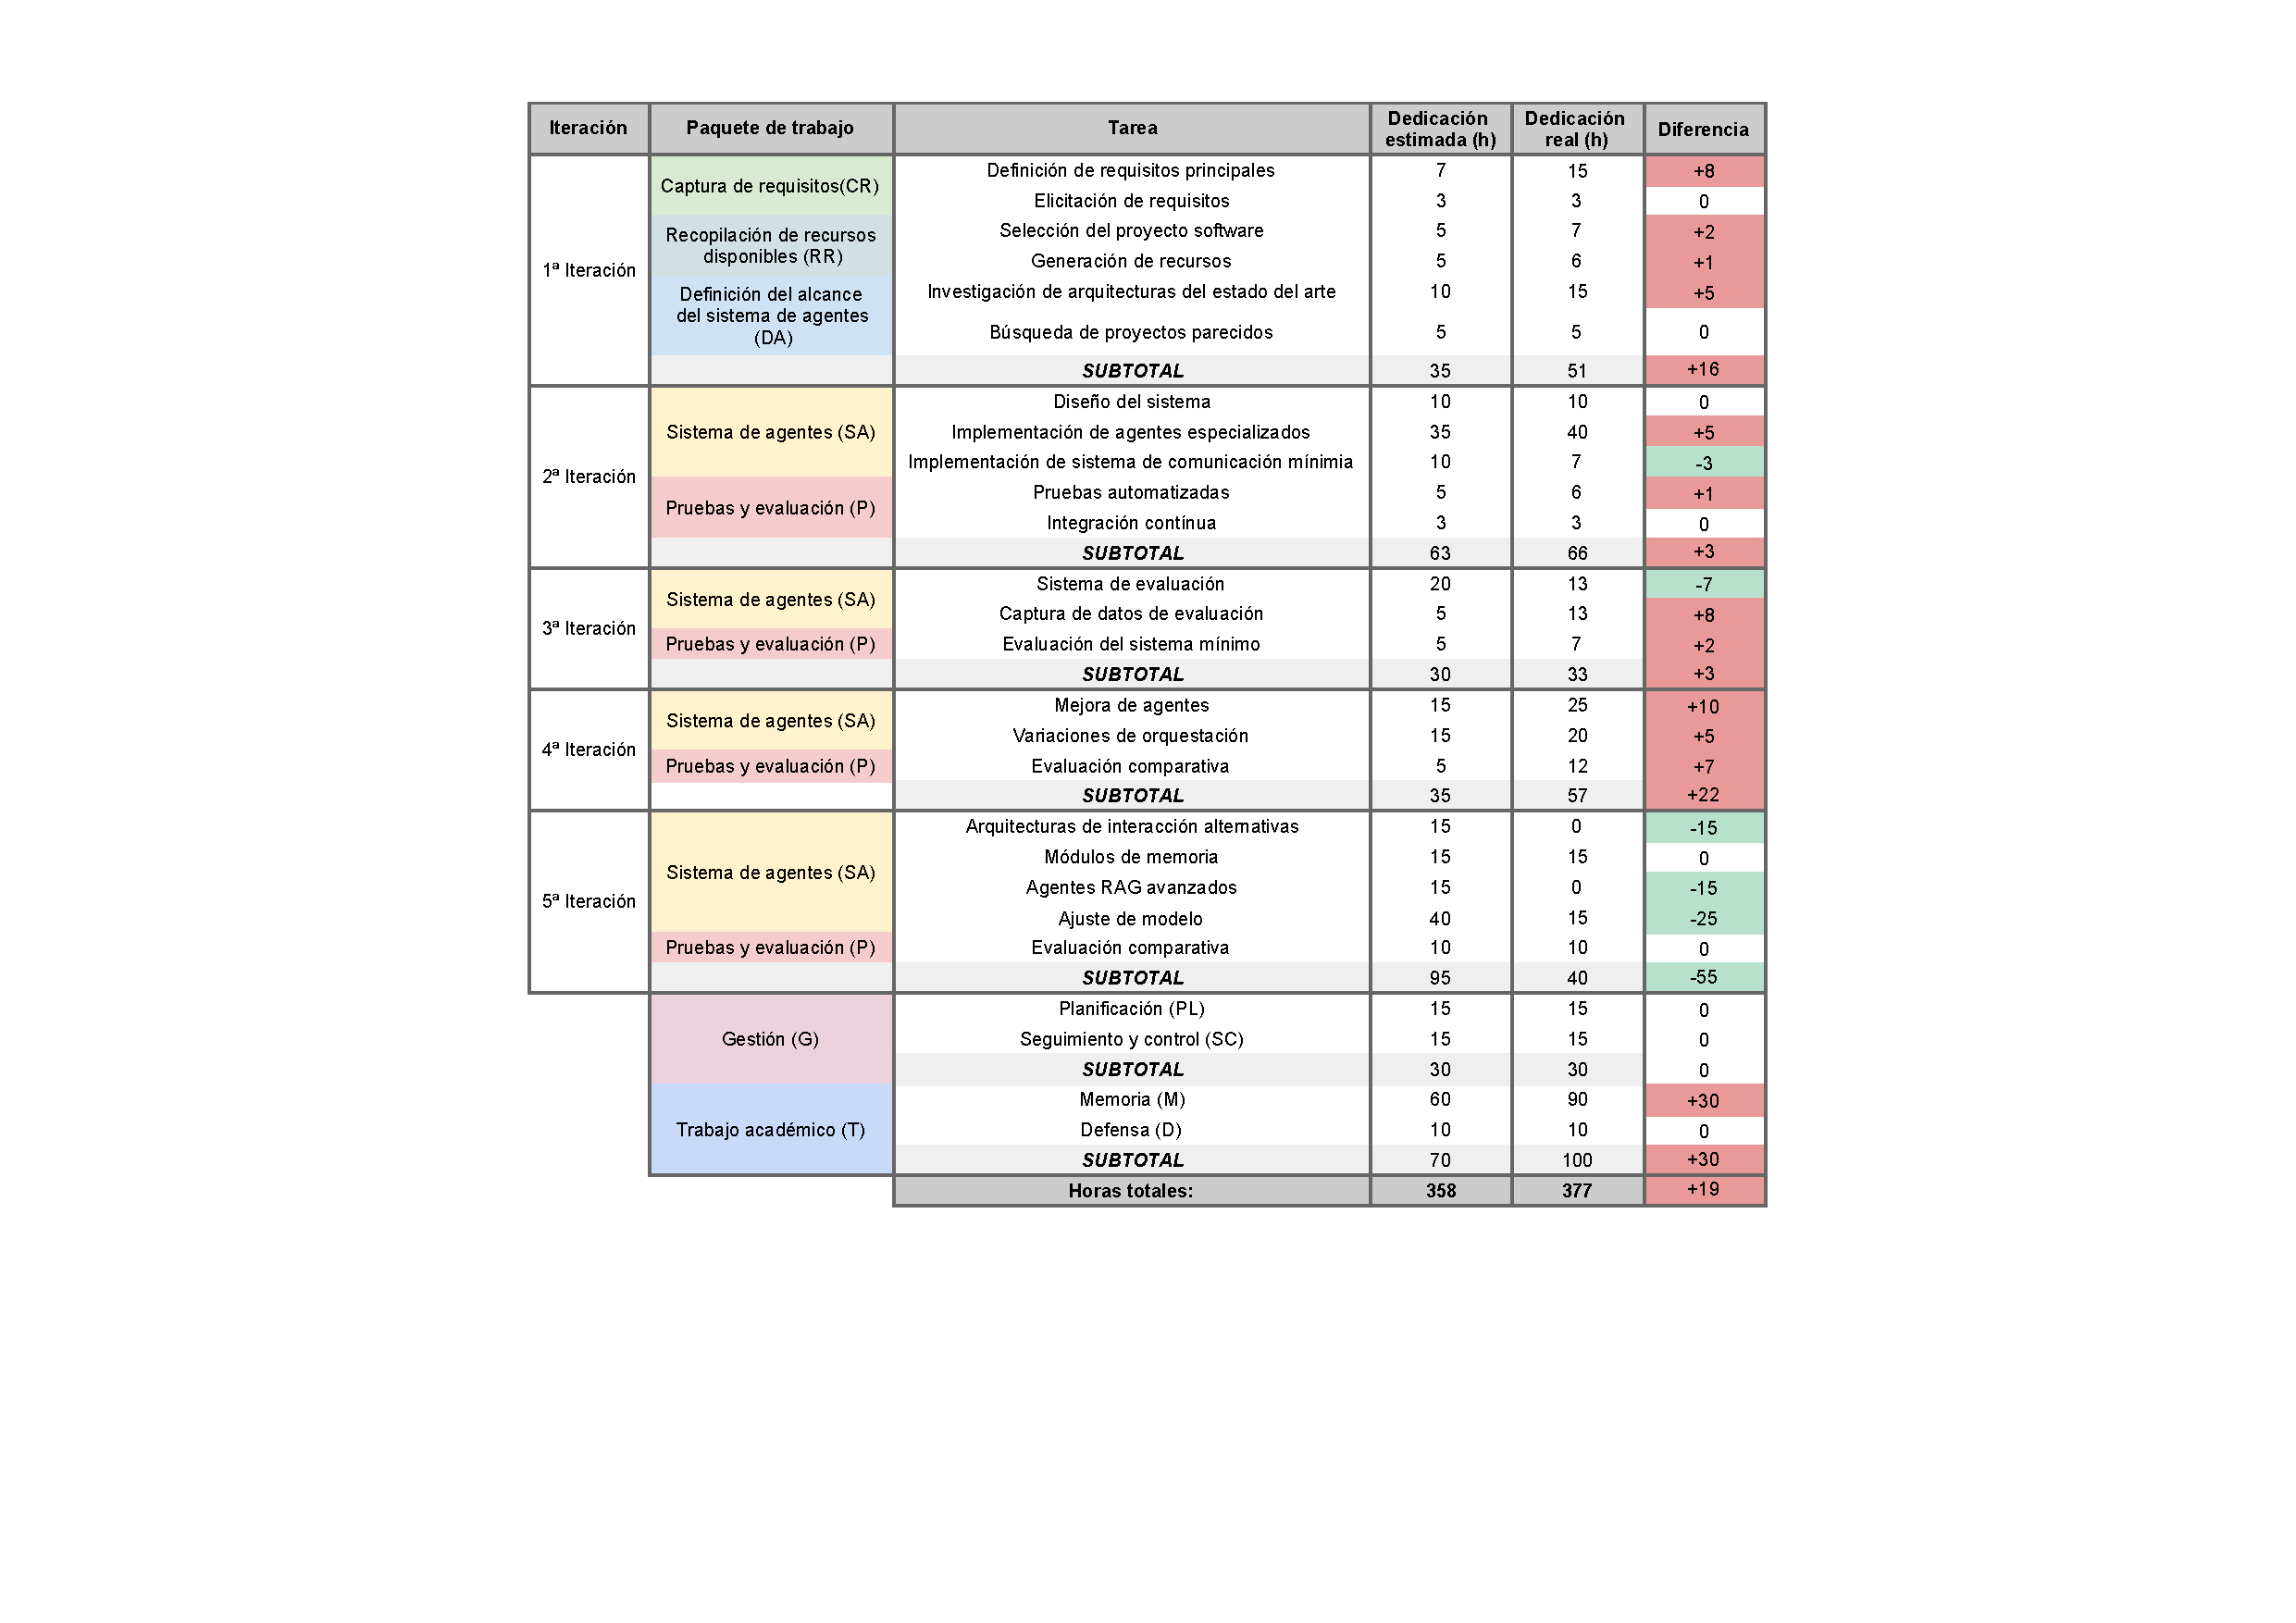
\includegraphics[width=1.25\linewidth]{figures/horas_real.pdf}}
\caption{Comparación de dedicación horaria estimada y real}
\label{fig:horas_real}
\end{figure}

El exceso horario en la primera iteración se debe principalmente a la dificultad para definir el alcance del sistema, lo cual implicó 16 horas adicionales o un 45\% de incremento.

La segunda y tercera iteraciones transcurrieron según lo planificado. Es destacable que la implementación del sistema de evaluación fue más sencilla de lo previsto, con 7 horas o un 35\% menor de dedicación, dado que el marco de evaluación de la librería LangSmith resultó conveniente e intuitivo. En cambio, la captura de datos de evaluación fue más compleja de lo esperado, requiriendo 8 horas adicionales o el 160\% de la tarea original.

La cuarta iteración fue también más compleja de lo esperado (+22 horas, +62\%), ya que se requirieron más correcciones del comportamiento inicial de lo previsto, necesitando 10 horas adicionales (60\%). La evaluación del sistema experimentó una desviación significativa de 10 horas o el 200\% de lo estimado, debido a que, aunque la evaluación estaba automatizada, fue necesario analizar las ejecuciones para sacar conclusiones y determinar los puntos a mejorar.

La dedicación a la última iteración fue aproximadamente la mitad de lo esperado debido a la reducción del alcance. El exceso de dedicación para la memoria ascendió a 30 horas o el 50\%, considerado razonable para la redacción de un documento que satisfaga los estándares académicos.

El sobrecoste total ha sido de 19 horas, equivalente al 5\% del proyecto.

